\documentclass[../../D1.tex]{subfiles}

\begin{document}
\emph{
- Discuss VPU/TPU/APU/GPU/FPGA/ASIC memory arcitecture and how it handles matrix sparsity\\
- Show ineffectivity of pruning on hardware without optimisations for sparse matrices\\
}
%The explosion of Deep Neural Network applications in recent years has prompted the production of a wave of specialised hardware architectures to improve the efficiency and compute of these kinds of workloads. The mainstay of this form of processing has been until recently been dominated by GPUs.\\


\subsubsection{Memory Allocation}\label{sec:MemAlloc}
\begin{figure}[H]
    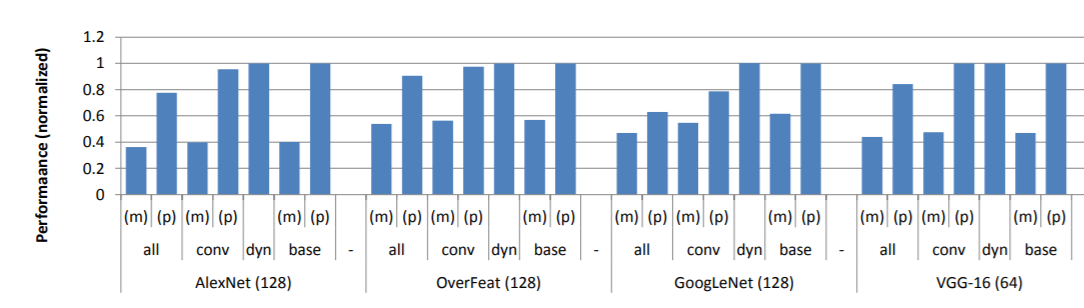
\includegraphics[width=1\textwidth]{vDNNperf.png} 
    \caption{vDNN performance, showing the throughput using various memory allocation strategies. \\ \textbf{(Adopted figure from~\autocite{rhuVDNNVirtualizedDeep2016})}}
    \label{fig:vDNNperf}   
\end{figure}
While designed specifically for training networks that would otherwise be to large for a GPU, the memory manager vDNN proposed in~\autocite{rhuVDNNVirtualizedDeep2016}~does provide some insight into the importance of memory locality to neural network throughput.
Fig.~\ref{fig:vDNNperf}~summarizes the performance of vDNN policies compared to a baseline memory management policy ($base$), the vDNN policies include: static policies (denoted as $all$ and $conv$) and a dynamic policy ($dyn$).
$base$ simply loads the full model into the GPU memory consequently providing optimal memory locality. $all$ refers to a policy of moving all $X$s out of GPU memory, and $conv$ only offloads $X$s from convolutional layers, $X$s are the input matrices to each layer, denoted by the red arrows in Fig.~\ref{fig:memAllocInf}.
Each of $base$, $conv$ and $all$ are evaluated using two distinct convolutional algorithms - memory-optimal ($m$) and performance-optimal ($p$).
Finally the $dyn$ allocation policy chooses ($m$) and ($p$) dynamically at runtime.
Fig.~\ref{fig:vDNNperf}~communicates a significant ($58\%$ and $55\%$) performance loss compared to baseline when no effort is made to optimise the memory locality of parameters in the network 

\begin{figure}[H]
    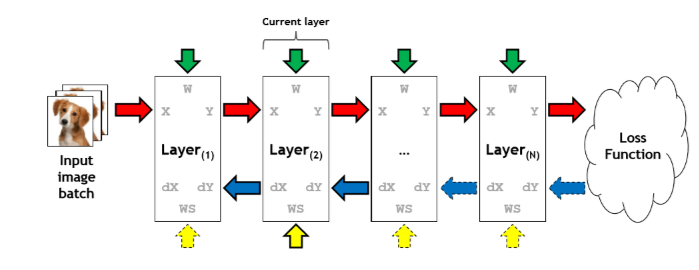
\includegraphics[width=1\textwidth]{MemoryAlloc.png} 
    \caption{Memory allocations required for linear networks. All green ($W$) and red ($X$) arrows are allocated during inference, the blue and yellow arrows are allocated during training.\\ \textbf{(Adopted figure from~\autocite{rhuVDNNVirtualizedDeep2016})}}
    \label{fig:memAllocInf}   
\end{figure}


Justifies the need for compression ... pruning


\subsubsection{Memory Access}
A significant portion of DNN computation is matrix-vector multiplication, the primary bottleneck of matrix-vector multiplication is memory access~\autocite{qiuGoingDeeperEmbedded2016}. 
When the cache capacity is insufficient for the input matrix size this bottleneck is expounded, as a consequence memory access is neccessary for every operation since there is no reuse of the input matrix~\autocite{hanEIEEfficientInference2016}.
% Need to rephase below see page 2 of EIEefficentInference paper
As observed in~\ref{sec:MemAlloc} this indicates that compression techniques should alliviate this bottleneck, and while compression doese reduce the total number of operations, the irregular memory access pattern caused by compression hinders effective acceleration see Fig.~\ref{fig:wallClockEIE}.

\begin{figure}[H]
    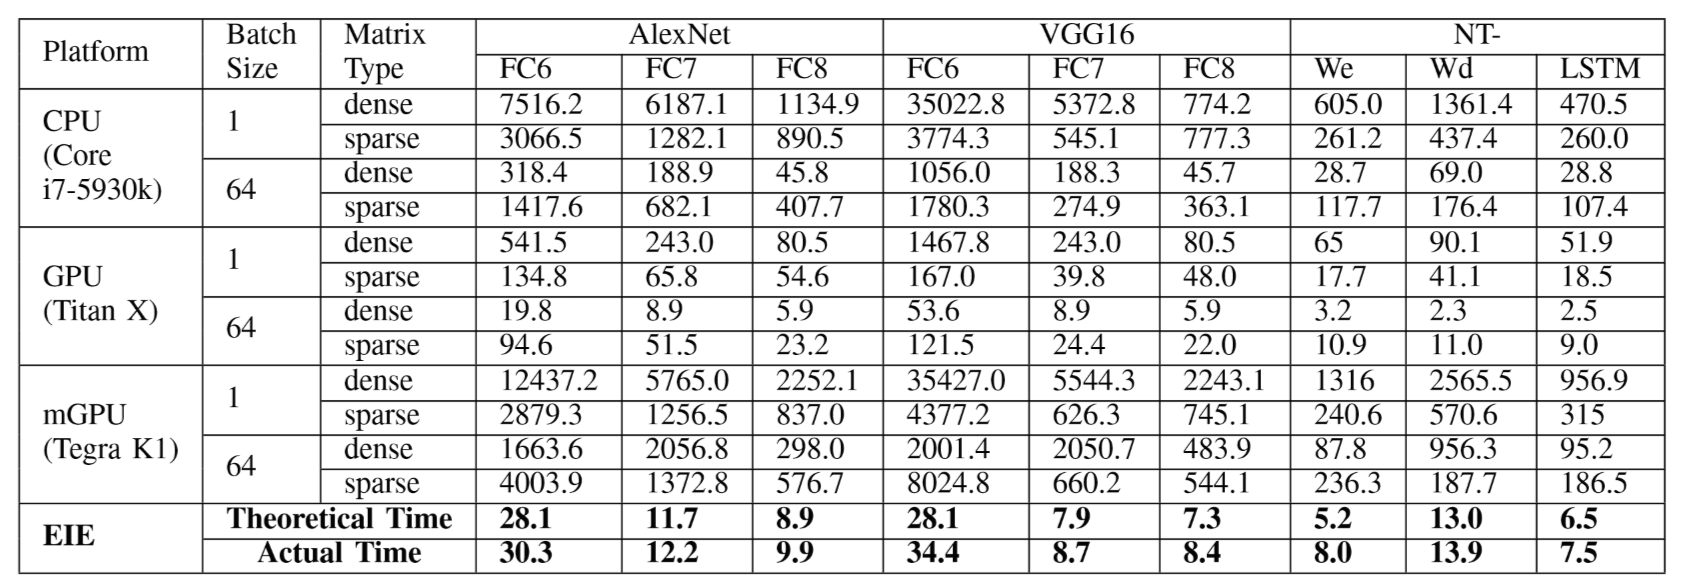
\includegraphics[width=1\textwidth]{wallClockEIE.png} 
    \caption{Wall clock time comparison for sparse and dense matrices between CPU, GPU, mGPU and EIE (an FPGA custom accelerator)\\ \textbf{(Adopted figure from~\autocite{hanEIEEfficientInference2016})}}
    \label{fig:wallClockEIE}   
\end{figure}

The paper proposing the EIE inference engine~\autocite{hanEIEEfficientInference2016} provides a clear description of a technique for exploiting the sparity of activations by storing an encoded sparse weight matrix in a variant of compressed sparse column format~\autocite{vuducAutomaticPerformanceTuning}.

\end{document}